\documentclass[a4paper,12pt]{article} % добавить leqno в [] для нумерации слева
\usepackage[a4paper,top=1.3cm,bottom=2cm,left=1.5cm,right=1.5cm,marginparwidth=0.75cm]{geometry}
%%% Работа с русским языком
\usepackage{cmap}					% поиск в PDF
\usepackage[warn]{mathtext} 		% русские буквы в фомулах
\usepackage[T2A]{fontenc}			% кодировка
\usepackage[utf8]{inputenc}			% кодировка исходного текста
\usepackage[english,russian]{babel}	% локализация и переносы
\usepackage{physics}
\usepackage{multirow}

%%% Нормальное размещение таблиц (писать [H] в окружении таблицы)
\usepackage{float}
\restylefloat{table}


\usepackage{graphicx}

\usepackage{wrapfig}
\usepackage{tabularx}

\usepackage{hyperref}
\usepackage[rgb]{xcolor}
\hypersetup{
	colorlinks=true,urlcolor=blue
}

%%% Дополнительная работа с математикой
\usepackage{amsmath,amsfonts,amssymb,amsthm,mathtools} % AMS
\usepackage{icomma} % "Умная" запятая: $0,2$ --- число, $0, 2$ --- перечисление

%% Номера формул
\mathtoolsset{showonlyrefs=true} % Показывать номера только у тех формул, на которые есть \eqref{} в тексте.

%% Шрифты
\usepackage{euscript}	 % Шрифт Евклид
\usepackage{mathrsfs} % Красивый матшрифт

%% Свои команды
\DeclareMathOperator{\sgn}{\mathop{sgn}}

%% Перенос знаков в формулах (по Львовскому)
\newcommand*{\hm}[1]{#1\nobreak\discretionary{}
	{\hbox{$\mathsurround=0pt #1$}}{}}

\date{\today}

\usepackage{gensymb}

\begin{document}

\begin{titlepage}
	\begin{center}
		{\large МОСКОВСКИЙ ФИЗИКО-ТЕХНИЧЕСКИЙ ИНСТИТУТ (НАЦИОНАЛЬНЫЙ ИССЛЕДОВАТЕЛЬСКИЙ УНИВЕРСИТЕТ)}
	\end{center}
	\begin{center}
		{\large Физтех-школа физики и исследований им. Ландау}
	\end{center}
	
	
	\vspace{4.5cm}
	{\huge
		\begin{center}
			{\bf Отчёт о выполнении лабораторной работы 2.2.4}\\
			Определение коэффициента теплопроводности твёрдых тел
		\end{center}
	}
	\vspace{2cm}
	\begin{flushright}
		{\LARGE Автор:\\ Сенокосов Арсений Олегович \\
			\vspace{0.2cm}
			Б02-012}
	\end{flushright}
	\vspace{8cm}
	\begin{center}
		Долгопрудный\\
		\today
	\end{center}
\end{titlepage}


\section{Введение}
\textbf{Цель работы:}  \begin{enumerate}
	\item определение коэффициентов теплопроводности твердых тел путем сравнения с теплопроводностью эталонного материала;
	\item вычисление относительных тепловых потерь через боковые поверхности по измеренным значениям температуры вдоль радиусов пластинок.
\end{enumerate}

\textbf{В работе используются:} термостат; набор термопар; зеркальный гальванометр; тонкие резиновые прокладки; исследуемые тела; диск из эталонного материала; штангенциркуль.

\section{Теоретические сведения:}

Количество теплоты $ \Delta q $, протекающее за единицу времени через однородную перегородку толщиной $ \Delta z $ и площадью $ S $ при разности температур $ \Delta T $, определяется формулой

\begin{equation}\label{osnova}
\Delta q = \varkappa S \frac{\Delta T}{\Delta z},
\end{equation}

где $ \varkappa $ -- коэффициент, характеризующий свойства среды и называемый коэффициентом теплопроводности.

Значение коэффициента теплопроводности $ \varkappa $ может быть определено непосредственно из формулы \eqref{osnova}, если измерить на опыте величины $ \Delta q $, $ \Delta T $, $ \Delta z $ и $ S $. Однако точное определение $ \varkappa $ с помощью формулы \eqref{osnova} оказывается нелегкой задачей из-за трудностей, возникающих при измерении количества теплоты. В настоящей работе вместо непосредственного измерения величины $ \varkappa $ произведём сравнение теплопроводности исследуемого материала с теплопроводностью некоторого другого эталонного материала с хорошо известным значением коэффициента $ \varkappa $. При этом можно избежать измерения $ \Delta q $. Идею метода поясняет рис. \ref{img:ust}.

Две пластинки, изготовленные из материалов с коэффициентами теплопроводности $ \varkappa_1 $ и $ \varkappa_2 $, зажимаются между стенками, температуры которых равны $ T_1 $ и $ T_2 $ и поддерживаются постоянными во время опыта. Если толщины пластинок $ d_1 $ и $ d_2 $ достаточно малы (по сравнению с наименьшим линейным размером их поверхности), то и потери тепла через боковые поверхности тоже малы. В таком случае площадь теплового потока, протекающего от горячей стенки к холодной, приблизительно остается постоянной. В этом случае

\begin{equation}\label{vivod}
\Delta q = \varkappa_1 S \frac{\Delta T_1}{\Delta z_1} = \varkappa_2 S \frac{\Delta T_2}{\Delta z_2}.
\end{equation}

Полагая, что $ \Delta z_1=d_1 $ и $ \Delta z_2=d_2 $, получим окончательно

\begin{equation}\label{itog}
\frac{\varkappa_1}{\varkappa_2} = \frac{d_1}{d_2}\frac{\Delta T_2}{\Delta T_1},
\end{equation}

где $ \Delta T_1 $ и $ \Delta T_2 $ -- перепады температур на пластинках. Зная теплопроводность материала одной из пластинок, легко определить на опыте теплопроводность другой пластинки.

Далее оценим размер тепловых потерь через боковые стороны исследуемого образца. Определим плотность радиального потока тепла $ q_r $. Эта величина определяется радиальным значением градиента температуры. Полный радиальный поток есть произведение $ q_r $ и площади боковой поверхности $ S_r $, вычисленной на том же расстоянии от оси симметрии, на котором производилось измерение радиальной производной температуры

\begin{equation}\label{poteri1}
q_r S_r = - \varkappa 2 \pi rd \frac{\partial T}{\partial r},
\end{equation}
где d -- толщина пластины.

Полный осевой поток определяется произведением производной температуры вдоль оси симметрии $ z $ и площади окружности, проходящей через точку измерения радиальной производной:

\begin{equation}\label{poteri2}
q_z S_z = - \varkappa \pi r^2 \frac{\partial T}{\partial z}.
\end{equation}

Отношение этих потоков обозначим $ \delta $:

\begin{equation}\label{poteri3}
\delta = \frac{2d \frac{\partial T}{\partial r}}{r \frac{\partial T}{\partial z}}.
\end{equation}

Этот параметр характеризует расширение теплового потока и его относительные потери, он не зависит от коэффициента теплопроводности.

Интересно отметить, что величина $ \delta $ не зависит и от радиуса, то есть отношение радиального потока к осевому одинаково и на оси симметрии, и вдали от неё. Расширение осевого теплового потока существует везде, а не только около краев пластинок. Это заключение следует из того, что температура имеет максимум на оси симметрии при любой координате z из-за симметрии пластинок. Поэтому разложение температуры по радиусу от оси начинается с квадратичного члена, следовательно, производная температуры по радиусу в формуле \eqref{poteri3} пропорциональна радиусу, и этот радиус сокращается с радиусом, который уже есть в знаменателе. Кроме того, при малых потерях через боковые стенки осевой поток тепла изменяется тоже на малую величину, поэтому, и производная $ \partial T/\partial z $ изменяется только на малую величину, то есть в первом приближении не зависит от радиуса как и остальные члены формулы \eqref{poteri3}. Отсюда можно сделать вывод, что относительное расширение теплового потока в однородной среде примерно одинаковое на всей пластинке.

\section{Экспериментальная установка}

\begin{figure}[H]
	\begin{center}
		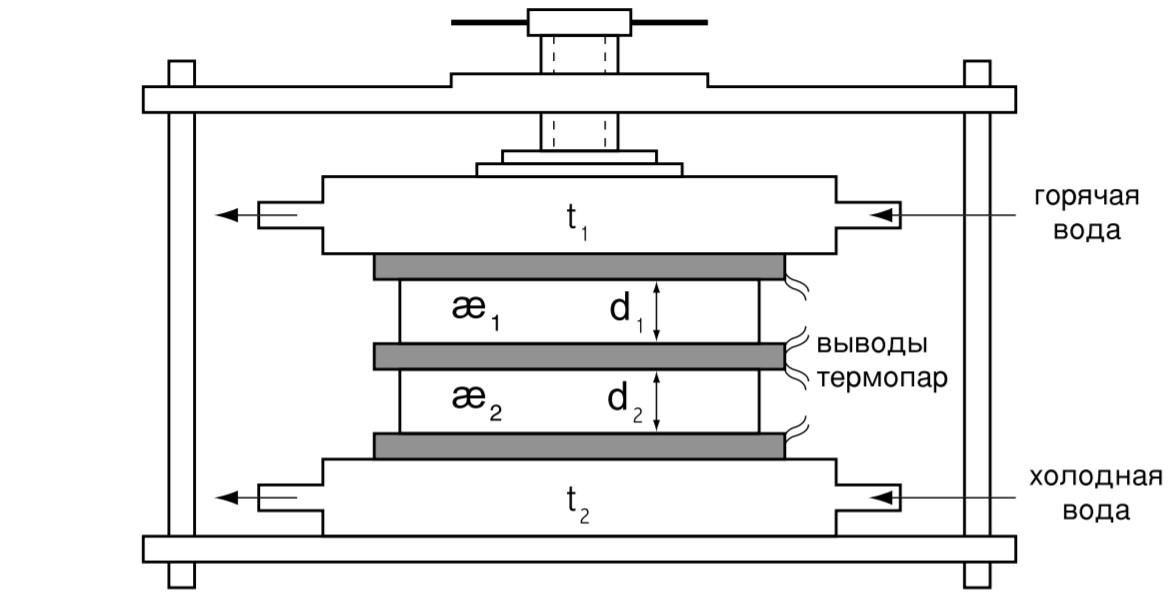
\includegraphics[width=15cm]{ust.jpg}
		\caption{Рисунок экспериментальной установки}\label{img:ust}
	\end{center}
\end{figure}

Прибор для измерения коэффициента теплопроводности (рис. \ref{img:ust}) представляет собой систему из нагревателя, имеющего температуру $ T_1 $, и холодильника, имеющего температуру $ T_2 $; эти температуры поддерживаются постоянными. Тепловой поток от нагревателя к холодильнику протекает через зажатые между ними пластинки из исследуемого и эталонного материала. 

В нашем приборе эталонным материалом является эбонит, коэффициент теплопроводности которого равен $ 0,17 $ Дж/м·с·К. Для получения надежного теплового контакта между поверхностями прокладывается резина. 

При измерениях коэффициента теплопроводности между нагревателем и холодильником закладываются переложенные тонкими резиновыми прокладками пластинки из исследуемого и эталонного материалов. Вся система сжимается винтовым прессом. 

Для стабилизации температур $ T_1 $ и $ T_2 $ через холодильник постоянно пропускается проточная вода из водопровода (вентиль на столе за прибором), а через нагреватель циркулирует горячая вода, поставляемая термостатом. Измерение температур производится при помощи четырех термопар, рабочие спаи которых помещают в середине пластинок. Спаи двух термопар прижимают резиновыми прокладками к обеим сторонам эталонной пластинки, спаи двух других -- к пластинке из исследуемого материала. Вторые спаи термопар помещены в пробирку с маслом, омываемую водопроводной водой. При этих условиях температура холодных спаев термопар за время эксперимент а практически не меняется.

\section{Ход работы}

\subsection{Оценка времени установления равновесия теплового потока}

Оценим время установления теплового равновесия. Снимем зависимость температуры фиксированной точки диска из эбонита от времени её измерения. Полученные данные занесём в таблицу \ref{tab:relaxation_time}.

\begin{table}[H]
	\centering
	\begin{tabular}{ccccccc}
		\hline
		\multicolumn{1}{|c|}{№ измерения} &
		\multicolumn{1}{c|}{1} &
		\multicolumn{1}{c|}{2} &
		\multicolumn{1}{c|}{3} &
		\multicolumn{1}{c|}{4} &
		\multicolumn{1}{c|}{5} &
		\multicolumn{1}{c|}{6} \\ \hline
		\multicolumn{1}{|c|}{$ t $, с} &
		\multicolumn{1}{c|}{10} &
		\multicolumn{1}{c|}{25} &
		\multicolumn{1}{c|}{40} &
		\multicolumn{1}{c|}{60} &
		\multicolumn{1}{c|}{80} &
		\multicolumn{1}{c|}{100} \\ \hline
		\multicolumn{1}{|c|}{$ U $, у.е.} &
		\multicolumn{1}{c|}{0,73} &
		\multicolumn{1}{c|}{0,76} &
		\multicolumn{1}{c|}{0,80} &
		\multicolumn{1}{c|}{0,86} &
		\multicolumn{1}{c|}{0,91} &
		\multicolumn{1}{c|}{0,91} \\ \hline
		&
		&
		&
		&
		&
		&
		\\ \hline
		\multicolumn{1}{|c|}{№ измерения} &
		\multicolumn{1}{c|}{7} &
		\multicolumn{1}{c|}{8} &
		\multicolumn{1}{c|}{9} &
		\multicolumn{1}{c|}{10} &
		\multicolumn{1}{c|}{11} &
		\multicolumn{1}{c|}{12} \\ \hline
		\multicolumn{1}{|c|}{$ t $, с} &
		\multicolumn{1}{c|}{130} &
		\multicolumn{1}{c|}{180} &
		\multicolumn{1}{c|}{220} &
		\multicolumn{1}{c|}{300} &
		\multicolumn{1}{c|}{400} &
		\multicolumn{1}{c|}{500} \\ \hline
		\multicolumn{1}{|c|}{$ U $, у.е.} &
		\multicolumn{1}{c|}{0,99} &
		\multicolumn{1}{c|}{1,05} &
		\multicolumn{1}{c|}{1,09} &
		\multicolumn{1}{c|}{1,13} &
		\multicolumn{1}{c|}{1,16} &
		\multicolumn{1}{c|}{1,18} \\ \hline
	\end{tabular}
	\caption{Зависимость температуры фиксированной точки от времени}
	\label{tab:relaxation_time}
\end{table}

По имеющимся экспериментальным данным построим график этой зависимости (рис. \ref{img:gr1}). 

\begin{figure}[H]
	\begin{center}
		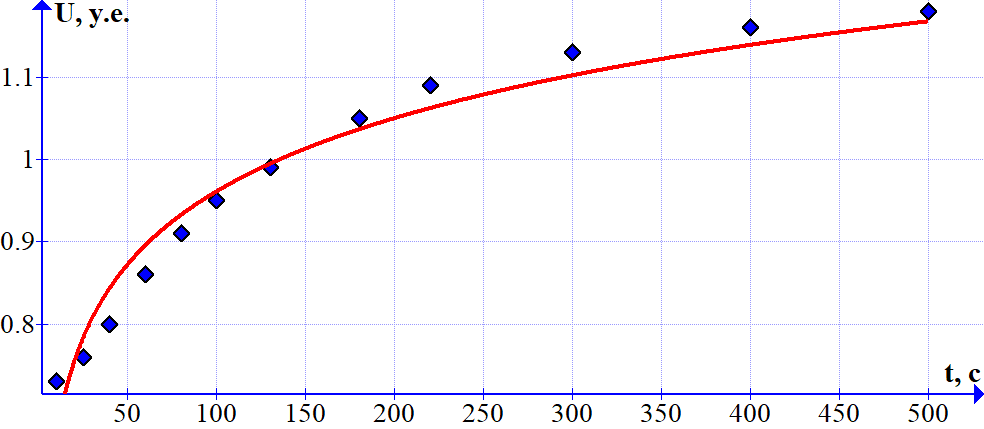
\includegraphics[width=17cm]{gr1.png}
		\caption{График зависимости температуры фиксированной точки от времени}\label{img:gr1}
	\end{center}
\end{figure}

Используя формулу, которая связывает распространение температуры в эбоните в зависимости от времени $ x^2 = t \chi $, где для эбонита $ \chi = 6 \cdot 10^{-8} $ $ \text{м}^2/\text{с} $ и $ x = d = 3,9 $ мм. Тогда время установления теплового равновесия \underline{$ t \approx  250$ с}.

Мы можем заметить, что оцененное теоретически время установления теплового равновесия с большой точностью совпадает с данными, полученными экспериментально. Значит в дальнейшем в ходе работы будем выжидать это время перед снятием показаний с гальванометра и считать, что после этого промежутка времени в системе установилось равновесие.

\subsection{Калибровка используемых термопар}

Прокалибруем применяемые в работе термопары. Для этого рабочие спаи термопар расположим в центре одной эбонитовой пластинки. После установления теплового равновесия в системе снимем показания с гальванометра. Полученные результаты занесём в таблицу \ref{tab:callib}.

\begin{table}[H]
	\centering
	\begin{tabular}{|c|c|}
		\hline
		$ \alpha_1 $, у.е. & 0,98 \\ \hline
		$ \alpha_2 $, у.е. & 0,98 \\ \hline
		$ \alpha_3 $, у.е. & 1,03 \\ \hline
		$ \alpha_4 $, у.е. & 0,94 \\ \hline
	\end{tabular}
	\caption{Показания термопар при измерении температуры фиксированной точки}
	\label{tab:callib}
\end{table}

Как можно заметить, показания гальванометра $ \alpha_1, \alpha_2, \alpha_3, \alpha_4 $ заметно отличаются друг от друга, поэтому отношение, входящее в формулу \eqref{itog}, будем вычислять по формуле

\begin{equation}\label{correction}
\frac{\Delta T_1}{\Delta T_2} = \frac{U_2/\alpha_2-U_1/\alpha_1}{U_4/\alpha_4-U_3/\alpha_3},
\end{equation}
где $ U_1, U_2, U_3, U_4 $ -- показания гальванометра, полученные во время опыта по измерению коэффициента теплопроводности. В этой формуле индексы при $ \alpha $ и $ U $ характеризуют номер термопары. Величины $ \alpha_i $ и $ U_i $ должны быть получены при подключении гальванометра к одной и той же термопаре.

\subsection{Проверка независимости коэффициента теплопроводности эбонита от температуры}

Проверим на опыте, в какой мере выполняется предположение о независимости коэффициента теплопроводности эталонного материала от температуры. Для этого в прибор зажмём пакет из двух одинаковых слоев пластинок эбонита, переложенных резиновыми прокладками. С помощью термопар измерим разности температур на эбонитовых слоях. Результаты измерения занесём в таблицу \ref{tab:free}.

\begin{table}[H]
	\centering
	\begin{tabular}{cc|l|l|}
		\cline{3-4}
		&  & $U_1$, у.е. & 0,21 \\ \cline{1-1} \cline{3-4} 
		\multicolumn{1}{|c|}{Эбонит} &  & $U_2$, у.е. & 1,16 \\ \cline{1-1} \cline{3-4} 
		\multicolumn{1}{|c|}{Эбонит} &  & $U_3$, у.е. & 1,17 \\ \cline{1-1} \cline{3-4} 
		&  & $U_4$, у.е. & 2,02 \\ \cline{3-4} 
	\end{tabular}\caption{Показания термопар в системе <<эбонит-эбонит>>}\label{tab:free}
\end{table}

Рассчитаем $ \Delta T_1 / \Delta T_2 $ по формуле \eqref{correction}. Получим \underline{$ \Delta T_1 / \Delta T_2 \approx 0,96 $.}

Используя формулы \label{formuli}\begin{align}
(\varepsilon_A)^2 = (\varepsilon_B)^2 + (\varepsilon_C)^2&, \quad A= B/C  \\  (\sigma_A)^2=(\sigma_B)^2+(\sigma_C)^2&, \quad A=B\pm C 
\end{align}
подсчитаем \[ \sigma_{\Delta T_1 / \Delta T_2} \approx 0,03 \].

Таким образом, получаем \[ \Delta T_1 / \Delta T_2 = 0,96\pm0,03 \quad \varepsilon = 0,04 \]
 

С помощью штангенциркуля измеряем толщину пластинок, измерения проводим несколько раз. В итоге получаем $ d_1 = d_2 = (3,9\pm0,1) $ мм. Этот результат был получен исходя ис того, что все измерения дали одинаковый результат, а значит случайная погрешность наших измерений пренебрежимо мала по сравнению с системной погрешностью, которую в данном случает примем равной цене деления штангенциркуля, т.е. $ 0,1 $ мм.

Исходя из полученных выше результатов можно утверждать, что $ d_1/d_2\approx\Delta T_1 / \Delta T_2 $. Таким образом, наше предположение о независимости коэффициента теплопроводности эбонита от температур в исследуемой области выполняется.

\subsection{Определение коэффициентов теплопроводности различных материалов}

Приступим к основному опыту. Измерим коэффициенты теплопроводности образцов (плексиглас, текстолит, гетинакс, стекло-текстолит). По показаниям гальванометра и по чувствительности термопар определим для каждого образца отношение разностей температур на образце и на эбоните согласно формуле \eqref{correction}, а затем используем формулу \eqref{itog}.

Для каждого образца проведём два измерения: один раз располагая образец со стороны нагревателя, а эталон — со стороны холодильника, а другой раз -- в обратном порядке. Полученные результаты занесём в таблицу \ref{tab:measurements}.

\begin{table}[H]
	\centering
	\begin{tabular}{ccccccccc}
		\cline{1-1} \cline{3-4} \cline{6-6} \cline{8-9}
		\multicolumn{1}{|c|}{$d = (3,9 \pm 0,1)$ мм} &
		\multicolumn{1}{c|}{} &
		\multicolumn{1}{c|}{$U_1$, у.е.} &
		\multicolumn{1}{c|}{0,28} &
		\multicolumn{1}{c|}{} &
		\multicolumn{1}{c|}{$d = (1,9 \pm 0,1)$ мм} &
		\multicolumn{1}{c|}{} &
		\multicolumn{1}{c|}{$U_1$, у.е.} &
		\multicolumn{1}{c|}{0,31} \\ \cline{1-1} \cline{3-4} \cline{6-6} \cline{8-9} 
		\multicolumn{1}{|c|}{Эбонит} &
		\multicolumn{1}{c|}{} &
		\multicolumn{1}{c|}{$U_2$, у.е.} &
		\multicolumn{1}{c|}{1,45} &
		\multicolumn{1}{c|}{} &
		\multicolumn{1}{c|}{Гетинакс} &
		\multicolumn{1}{c|}{} &
		\multicolumn{1}{c|}{$U_2$, у.е.} &
		\multicolumn{1}{c|}{0,93} \\ \cline{1-1} \cline{3-4} \cline{6-6} \cline{8-9} 
		\multicolumn{1}{|c|}{Гетинакс} &
		\multicolumn{1}{c|}{} &
		\multicolumn{1}{c|}{$U_3$, у.е.} &
		\multicolumn{1}{c|}{1,48} &
		\multicolumn{1}{c|}{} &
		\multicolumn{1}{c|}{Эбонит} &
		\multicolumn{1}{c|}{} &
		\multicolumn{1}{c|}{$U_3$, у.е.} &
		\multicolumn{1}{c|}{0,96} \\ \cline{1-1} \cline{3-4} \cline{6-6} \cline{8-9} 
		\multicolumn{1}{|c|}{$d = (1,9 \pm 0,1)$ мм} &
		\multicolumn{1}{c|}{} &
		\multicolumn{1}{c|}{$U_4$, у.е.} &
		\multicolumn{1}{c|}{2,03} &
		\multicolumn{1}{c|}{} &
		\multicolumn{1}{c|}{$d = (3,9 \pm 0,1)$ мм} &
		\multicolumn{1}{c|}{} &
		\multicolumn{1}{c|}{$U_4$, у.е.} &
		\multicolumn{1}{c|}{1,98} \\ \cline{1-1} \cline{3-4} \cline{6-6} \cline{8-9} 
		&
		&
		&
		&
		&
		&
		&
		&
		\\ \cline{1-1} \cline{3-4} \cline{6-6} \cline{8-9} 
		\multicolumn{1}{|c|}{$d = (3,9 \pm 0,1)$ мм} &
		\multicolumn{1}{c|}{} &
		\multicolumn{1}{c|}{$U_1$, у.е.} &
		\multicolumn{1}{c|}{0,28} &
		\multicolumn{1}{c|}{} &
		\multicolumn{1}{c|}{$d = (4,8 \pm 0,1)$ мм} &
		\multicolumn{1}{c|}{} &
		\multicolumn{1}{c|}{$U_1$, у.е.} &
		\multicolumn{1}{c|}{0,24} \\ \cline{1-1} \cline{3-4} \cline{6-6} \cline{8-9} 
		\multicolumn{1}{|c|}{Эбонит} &
		\multicolumn{1}{c|}{} &
		\multicolumn{1}{c|}{$U_2$, у.е.} &
		\multicolumn{1}{c|}{1,05} &
		\multicolumn{1}{c|}{} &
		\multicolumn{1}{c|}{Плексиглас} &
		\multicolumn{1}{c|}{} &
		\multicolumn{1}{c|}{$U_2$, у.е.} &
		\multicolumn{1}{c|}{1,24} \\ \cline{1-1} \cline{3-4} \cline{6-6} \cline{8-9} 
		\multicolumn{1}{|c|}{Плексиглас} &
		\multicolumn{1}{c|}{} &
		\multicolumn{1}{c|}{$U_3$, у.е.} &
		\multicolumn{1}{c|}{1,12} &
		\multicolumn{1}{c|}{} &
		\multicolumn{1}{c|}{Эбонит} &
		\multicolumn{1}{c|}{} &
		\multicolumn{1}{c|}{$U_3$, у.е.} &
		\multicolumn{1}{c|}{1,27} \\ \cline{1-1} \cline{3-4} \cline{6-6} \cline{8-9} 
		\multicolumn{1}{|c|}{$d = (4,8 \pm 0,1)$ мм} &
		\multicolumn{1}{c|}{} &
		\multicolumn{1}{c|}{$U_4$, у.е.} &
		\multicolumn{1}{c|}{2,01} &
		\multicolumn{1}{c|}{} &
		\multicolumn{1}{c|}{$d = (3,9 \pm 0,1)$ мм} &
		\multicolumn{1}{c|}{} &
		\multicolumn{1}{c|}{$U_4$, у.е.} &
		\multicolumn{1}{c|}{2,02} \\ \cline{1-1} \cline{3-4} \cline{6-6} \cline{8-9} 
		&
		&
		&
		&
		&
		&
		&
		&
		\\ \cline{1-1} \cline{3-4} \cline{6-6} \cline{8-9} 
		\multicolumn{1}{|c|}{$d = (3,9 \pm 0,1)$ мм} &
		\multicolumn{1}{c|}{} &
		\multicolumn{1}{c|}{$U_1$, у.е.} &
		\multicolumn{1}{c|}{0,26} &
		\multicolumn{1}{c|}{} &
		\multicolumn{1}{c|}{$d = (3,9 \pm 0,1)$ мм} &
		\multicolumn{1}{c|}{} &
		\multicolumn{1}{c|}{$U_1$, у.е.} &
		\multicolumn{1}{c|}{0,32} \\ \cline{1-1} \cline{3-4} \cline{6-6} \cline{8-9} 
		\multicolumn{1}{|c|}{Эбонит} &
		\multicolumn{1}{c|}{} &
		\multicolumn{1}{c|}{$U_2$, у.е.} &
		\multicolumn{1}{c|}{1,29} &
		\multicolumn{1}{c|}{} &
		\multicolumn{1}{c|}{Текстолит} &
		\multicolumn{1}{c|}{} &
		\multicolumn{1}{c|}{$U_2$, у.е.} &
		\multicolumn{1}{c|}{1,15} \\ \cline{1-1} \cline{3-4} \cline{6-6} \cline{8-9} 
		\multicolumn{1}{|c|}{Текстолит} &
		\multicolumn{1}{c|}{} &
		\multicolumn{1}{c|}{$U_3$, у.е.} &
		\multicolumn{1}{c|}{1,32} &
		\multicolumn{1}{c|}{} &
		\multicolumn{1}{c|}{Эбонит} &
		\multicolumn{1}{c|}{} &
		\multicolumn{1}{c|}{$U_3$, у.е.} &
		\multicolumn{1}{c|}{1,17} \\ \cline{1-1} \cline{3-4} \cline{6-6} \cline{8-9} 
		\multicolumn{1}{|c|}{$d = (3,9 \pm 0,1)$ мм} &
		\multicolumn{1}{c|}{} &
		\multicolumn{1}{c|}{$U_4$, у.е.} &
		\multicolumn{1}{c|}{2,01} &
		\multicolumn{1}{c|}{} &
		\multicolumn{1}{c|}{$d = (3,9 \pm 0,1)$ мм} &
		\multicolumn{1}{c|}{} &
		\multicolumn{1}{c|}{$U_4$, у.е.} &
		\multicolumn{1}{c|}{2,07} \\ \cline{1-1} \cline{3-4} \cline{6-6} \cline{8-9} 
		&
		&
		&
		&
		&
		&
		&
		&
		\\ \cline{1-1} \cline{3-4} \cline{6-6} \cline{8-9} 
		\multicolumn{1}{|c|}{$d = (3,9 \pm 0,1)$ мм} &
		\multicolumn{1}{c|}{} &
		\multicolumn{1}{c|}{$U_1$, у.е.} &
		\multicolumn{1}{c|}{0,32} &
		\multicolumn{1}{c|}{} &
		\multicolumn{1}{c|}{$d = (1,6 \pm 0,1)$ мм} &
		\multicolumn{1}{c|}{} &
		\multicolumn{1}{c|}{$U_1$, у.е.} &
		\multicolumn{1}{c|}{0,39} \\ \cline{1-1} \cline{3-4} \cline{6-6} \cline{8-9} 
		\multicolumn{1}{|c|}{Эбонит} &
		\multicolumn{1}{c|}{} &
		\multicolumn{1}{c|}{$U_2$, у.е.} &
		\multicolumn{1}{c|}{1,63} &
		\multicolumn{1}{c|}{} &
		\multicolumn{1}{c|}{Ст.-текстолит} &
		\multicolumn{1}{c|}{} &
		\multicolumn{1}{c|}{$U_2$, у.е.} &
		\multicolumn{1}{c|}{0,98} \\ \cline{1-1} \cline{3-4} \cline{6-6} \cline{8-9} 
		\multicolumn{1}{|c|}{Ст.-текстолит} &
		\multicolumn{1}{c|}{} &
		\multicolumn{1}{c|}{$U_3$, у.е.} &
		\multicolumn{1}{c|}{1,64} &
		\multicolumn{1}{c|}{} &
		\multicolumn{1}{c|}{Эбонит} &
		\multicolumn{1}{c|}{} &
		\multicolumn{1}{c|}{$U_3$, у.е.} &
		\multicolumn{1}{c|}{1,01} \\ \cline{1-1} \cline{3-4} \cline{6-6} \cline{8-9} 
		\multicolumn{1}{|c|}{$d = (1,6 \pm 0,1)$ мм} &
		\multicolumn{1}{c|}{} &
		\multicolumn{1}{c|}{$U_4$, у.е.} &
		\multicolumn{1}{c|}{2,08} &
		\multicolumn{1}{c|}{} &
		\multicolumn{1}{c|}{$d = (3,9 \pm 0,1)$ мм} &
		\multicolumn{1}{c|}{} &
		\multicolumn{1}{c|}{$U_4$, у.е.} &
		\multicolumn{1}{c|}{2,09} \\ \cline{1-1} \cline{3-4} \cline{6-6} \cline{8-9} 
	\end{tabular}
	\caption{Результаты измерения физических данных}
	\label{tab:measurements}
\end{table}

В таблице над каждым образцом указана его толщина. Эти измерения проводились штангенциркулем многократно для каждого образца. При этих измерения получались одинаковые данные, поэтому случайной погрешностью измерений можно пренебречь.

При снятии показаний с гальванометра за систематическую ошибку можно принять цену деления, т.е. $\sigma_U^\text{сист} = 0,1 $ у.е.

При вычислении коэффициента теплопроводности исследуемого материала по формуле \eqref{itog} также вычисляем погрешность полученных результатов по формуле ниже:

\begin{equation}\label{pogr}
\varepsilon_\varkappa = \sqrt{\varepsilon^2_{d_1} + \varepsilon^2_{d_2} + \varepsilon^2_{\Delta T_1/\Delta T_2}}
\end{equation}

Для расчёта $ \varepsilon_{\Delta T_1/\Delta T_2} $ используем формулы, приведённые в п. \ref{formuli}.

Кроме значений $ \varkappa $ для каждого отдельного опыта также вычислим среднее значение коэффициента теплопроводности $ \left<\varkappa\right> $ для каждого материала. Вычисления проведём по формулам: \[ \left< \varkappa \right> = \frac{\varkappa_\text{хол}+\varkappa_\text{нагр}}{2}; \] 
\[ \sigma_{\left<\varkappa\right>}^{\text{сист}} \approx \sigma_\varkappa; \]
\[ \sigma_{\left<\varkappa\right>}^{\text{случ}} = \sqrt{\frac{1}{2}\sum_{i=1}^{2}\left(\varkappa_i-\left<\varkappa\right>\right)^2}; \]
\[ \sigma_{\left<\varkappa\right>} = \sqrt{\sigma^2_{\text{сист}}+\sigma^2_{\text{случ}}}. \]

Полученные результаты заносим в таблицу \ref{tab:result2}.

% Please add the following required packages to your document preamble:
% \usepackage{multirow}
\begin{table}[H]
	\centering
	\begin{tabular}{|c|c|c|c|c|c|c|c|}
		\hline
		Материал                       & Режим измерения &$ \varkappa $, $ \frac{\text{Вт}}{\text{м} \cdot \text{с}} $    & $ \sigma_\varkappa $, $ \frac{\text{Вт}}{\text{м} \cdot \text{с}} $ & $ \varepsilon_\varkappa $, \% & $ \left<\varkappa\right> $, $ \frac{\text{Вт}}{\text{м} \cdot \text{с}} $                  & $ \sigma_{\left<\varkappa\right>} $, $ \frac{\text{Вт}}{\text{м} \cdot \text{с}} $            & $ \varepsilon_{\left<\varkappa\right>} $, \%           \\ \hline
		\multirow{2}{*}{Гетинакс}      & нагреватель     & 0,137 & 0,010    & 7,43     & \multirow{2}{*}{0,145} & \multirow{2}{*}{0,013} & \multirow{2}{*}{9,23} \\ \cline{2-5}
		& холодильник & 0,154 & 0,011 & 6,92 &  &  &  \\ \hline
		\multirow{2}{*}{Плексиглас}    & нагреватель     & 0,158 & 0,008    & 4,88     & \multirow{2}{*}{0,173} & \multirow{2}{*}{0,017} & \multirow{2}{*}{9,81} \\ \cline{2-5}
		& холодильник & 0,188 & 0,009 & 5,00 &  &  &  \\ \hline
		\multirow{2}{*}{Текстолит}     & нагреватель     & 0,209 & 0,011    & 5,20     & \multirow{2}{*}{0,211} & \multirow{2}{*}{0,011} & \multirow{2}{*}{5,30} \\ \cline{2-5}
		& холодильник & 0,214 & 0,011 & 5,09 &  &  &  \\ \hline
		\multirow{2}{*}{Ст.-текстолит} & нагреватель     & 0,150 & 0,013    & 8,63     & \multirow{2}{*}{0,147} & \multirow{2}{*}{0,012} & \multirow{2}{*}{8,48} \\ \cline{2-5}
		& холодильник & 0,144 & 0,011 & 7,76 &  &  &  \\ \hline
	\end{tabular}
	\caption{Результаты вычисления коэффициентов теплопроводности различных материалов}
	\label{tab:result2}
\end{table}

Итого получаем:

\begin{itemize}
	\item гетинакс: $ \varkappa = (0,145 \pm 0,013) $ $ \frac{\text{Вт}}{\text{м} \cdot \text{с}} $, ($\varepsilon = 9,2\%$)
	\item плексиглас: $ \varkappa = (0,173 \pm 0,017) $ $ \frac{\text{Вт}}{\text{м} \cdot \text{с}} $, ($\varepsilon = 9,8\%$)
	\item текстолит: $ \varkappa = (0,211 \pm 0,011) $ $ \frac{\text{Вт}}{\text{м} \cdot \text{с}} $, ($\varepsilon = 5,3\%$)
	\item ст.-текстолит: $ \varkappa = (0,147 \pm 0,012) $ $ \frac{\text{Вт}}{\text{м} \cdot \text{с}} $, ($\varepsilon = 8,5\%$)
\end{itemize}

\subsection{Оценка тепловых потерь через боковые стороны}

Оценим потери через боковые поверхности. Разместим рабочие спаи термопар на разных расстояниях от центра пластины. Чтобы избежать ошибок, связанных с теплоотводом через провода термопар в этом точном эксперименте, длины всех прижатых частей проводов сделаем одинаковыми. С помощью гальванометра измерим температуры всех спаев и результаты измерений (делённые на соответствующую чувствительность) занесём в таблицу \ref{tab:losses}.

\begin{table}[H]
	\centering
	\begin{tabular}{|l|l|l|}
		\hline
		$ r $, мм & $ U $, у.е. & $ U/\alpha $  \\ \hline
		1,1   & 1,16    & 1,18 \\ \hline
		9,7   & 1,14    & 1,16 \\ \hline
		24,1  & 1,1     & 1,07 \\ \hline
		42,6  & 0,88    & 0,94 \\ \hline
	\end{tabular}
	\caption{Измерение распределения температур}
	\label{tab:losses}
\end{table}

Построим график зависимости от радиуса показаний гальванометра, поделенных на чувствительность каждой термопары (см. рис. \ref{img:gr2}). 

\begin{figure}[H]
	\begin{center}
		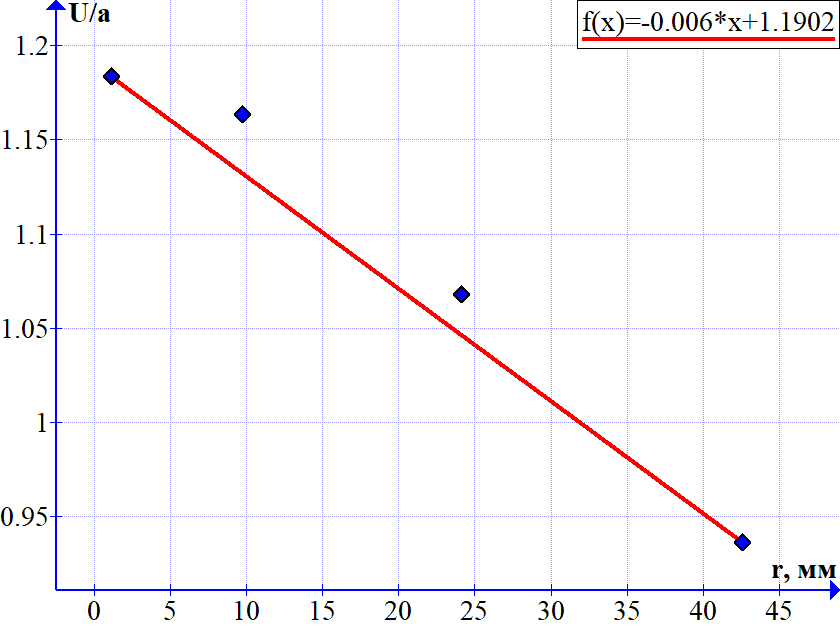
\includegraphics[width=17cm]{gr2.png}
		\caption{График зависимости температуры от расстояния до центра образца}\label{img:gr2}
	\end{center}
\end{figure}

Уменьшение температуры при удалении от центра обусловлено тепловым потоком через боковые поверхности. По графику найдём производную температуры по радиусу.

Так как распределение температуры по радиусы близко к параболическому, то производная в точке $ r = 42,6 $ мм в два раза больше производной для прямой, соединяющей температуру в этой точке с температурой в центре пластины.

Отсюда получаем \[ \frac{\partial T}{\partial r} = 2 \cdot (-0,006) = -0,012 \text{ у.е./мм}. \]

Из опытов с эбонитовой пластинкой в прошлых экспериментах получаем, что

\[ \frac{\partial T}{\partial z} = 0,303 \text{ у.е./мм}. \]

При этом радиус исследуемого образца равен $r = 50,4 $ мм, он был измерен при помощи штангенциркуля.

Тогда по формуле \eqref{poteri3} \[ \delta = \frac{2d \frac{\partial T}{\partial r}}{r \frac{\partial T}{\partial z}}  \approx 6,13 \cdot 10^{-3}. \]

Таким образом величина относительных потерь составляет $ \delta = 0,6 \%$, что подтверждает малось радиального теплового потока по сравнению с осевым.

\section{Обсуждение результатов и выводы}

\begin{itemize}
	\item Во время выполнения работы было экспериментально измерено время установления теплового равновесия, оно составило $ \approx 300 $ секунд
	\item Полученное экспериментально время установления теплового равновесия оказалось близко ко времени, рассчитанному теоретически
	\item В ходе работы были прокалиброваны используемые термопары, чтобы полученные результаты были корректны
	\item В работе была экспериментально подтверждена гипотеза о независимости коэффициента теплопроводности эталонного материала (эбонита) от температуры в пределах от $ 10\degree $C до $ 70\degree $C
	\item В работе был измерен коэффициент теплопроводности четырёх различных материалов. По полученным результатом можно судить о независимости коэффициентов теплопроводности этих материалов при исследуемой температуре
	\begin{itemize}
		\item гетинакс: $ \varkappa = (0,145 \pm 0,013) $ $ \frac{\text{Вт}}{\text{м} \cdot \text{с}} $, ($\varepsilon = 9,2\%$)
		\item плексиглас: $ \varkappa = (0,173 \pm 0,017) $ $ \frac{\text{Вт}}{\text{м} \cdot \text{с}} $, ($\varepsilon = 9,8\%$)
		\item текстолит: $ \varkappa = (0,211 \pm 0,011) $ $ \frac{\text{Вт}}{\text{м} \cdot \text{с}} $, ($\varepsilon = 5,3\%$)
		\item ст.-текстолит: $ \varkappa = (0,147 \pm 0,012) $ $ \frac{\text{Вт}}{\text{м} \cdot \text{с}} $, ($\varepsilon = 8,5\%$)
	\end{itemize}
	\item Также в ходе работы была проведена оценка радиальных тепловых потерь. В результате было получено, что величина относительных потерь составляет $ \delta \approx 0,6\% $. Полученный результат говорит о их малости
\end{itemize}

В ходе выполнения работы нельзя было избежать ошибок, связанных с методом измерений. Основную погрешность вносили тепловые потери через боковые стороны установки, потери тепла через провода используемых термопар. Также свой вклад в погрешность внесли используемые в работе резиновые прокладки, поскольку материал, из которого они изготовлены не является идеальным тепло-проводником.

Для повышения точности измерений можно обложить установку теплоизолирующим материалом. Также лучше фиксировать место положение термопар, чтобы избежать их смещения в процессе закрепления исследуемого образца.




\end{document}